
\documentclass[journal,12pt,twocolumn]{IEEEtran}
\usepackage{amsfonts}  %% 010
\usepackage{amsmath}  %% 010
\usepackage{amssymb,amsmath,mathtools,xcolor,graphicx,xspace,colortbl,ragged2e,rotating}  %% 100
\usepackage{boxedminipage}  %% 100
\usepackage{graphics}  %% 100
\usepackage{ragged2e}  %% 100
\usepackage{wrapfig}  %% 100
\usepackage{xcolor}  %% 200
\graphicspath{{images/}}
\DeclareGraphicsExtensions{.pdf,.eps,.ps,.png,.jpg,.jpeg}
\begin{document}
\title{\textbf{AI1110 Assignment 1} }
\author{\textbf{Dondapati Chandrahas Reddy}\\\textbf{AI21BTECH11010}}
\maketitle
\begin{center}
{ ICSE Grade 10 2019 paper}\end{center}\par
{ \section {Question 3 (a) \newline}}
{\Large \underline{Question}:}


\begin{center}
\setlength \fboxrule {0in}
\setlength \fboxsep {0.1in}
\fcolorbox[HTML]{FFFFFF}{FFFFFF}{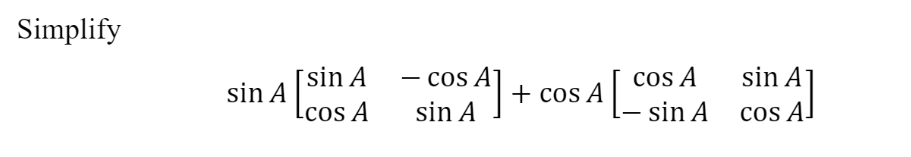
\includegraphics [ width=5.8125in, height=1in,]{img1} }
\end{center}\par

{\Large \underline{Solution}: \newline\newline }\par
Let,
\begin{center}$R =\left [\begin{array}{cc}\cos A &  -\sin A \\
\sin A & \cos A\end{array}\right ]$\newline\end{center}\par

The matrix expression in the question can be written as

\begin{center}
$\sin A\left [\begin{array}{cc}0 &  -1 \\
1 & 0\end{array}\right ]R^{ -1} +\cos A \ast R^{ -1}$\newline 
\end{center}\par

Taking $R^{ -1}$ common

\begin{center}
$\left (\sin A\left [\begin{array}{cc}0 &  -1 \\
1 & 0^{}\end{array}\right ] +\cos A\left [\begin{array}{cc}1 & 0 \\
0 & 1\end{array}\right ]\right )R^{ -1}$\newline
\end{center}\par

Simplifying the expression

\begin{center}
$\left [\begin{array}{cc}\cos A &  -\sin A \\
\sin A & \cos A\end{array}\right ]R^{ -1}$\linebreak\relax
\end{center}\par

Multiplying the matrices finally gives

\begin{center}
$\left [\begin{array}{cc}1 & 0 \\
0 & 1\end{array}\right ]$
\end{center}\par
\end{document}